% !TeX root = ../main.tex
% Add the above to each chapter to make compiling the PDF easier in some editors.

\chapter{Dataset}\label{chapter:dataset}

This thesis aims to develop a compressed sensing framework that leverages the strengths of deep generative models.
Methods proposed by \textcite{CSUsingAI} have demonstrated superior reconstructions with fewer measurements than classical compressed sensing techniques.
Consequently, this thesis focuses on reconstructing ill-posed problems with many unknowns.

Datasets with high spatial resolution inventories are required to facilitate this.
Datasets like CAMS-REG-v4 \parencite{CAMS} provide \gls{GHG} emissions at a resolution of $0.1^{\circ}$ latitude by $0.05^{\circ}$ longitude, which corresponds to approximately $5$ by $5$ kilometers over central Europe.
This resolution is relatively low.
For example, a city spanning a $30 \unit{km}$ by $30 \unit{km}$ area would be divided into a spatial grid of $6$ by $6$ cells.
Therefore, this thesis utilizes the high-resolution inventories TNO-GHGco-v1.1 for $2015$ emissions \parencite{TNO_HighRes15} and TNO-GHGco-v4 for $2018$ emissions \parencite{TNO_HighRes18}.
These inventories provide emissions at spatial resolution of ${{}^{1}\!/\!{}_{120}}^\circ$ latitude by ${{}^{1}\!/\!{}_{60}}^\circ$ longitude, or approximately $1 \unit{km}$ by $1 \unit{km}$.
This high spatial resolution allows for extracting detailed emission fields in urban environments.
The inventories include \gls{GHG} emissions for each GNFR sector, with the road sector (sector F) further divided into four subsectors, for each coordinate in a defined European grid.
This results in $15$ emission values per gas per cell.

In this thesis, only $\text{CO}_2$ emissions from fossil fuels (ff) are considered.
However, the approaches presented can be directly applied to all \gls{GHG} sources.
Furthermore, as point sources are assumed to be known, only diffuse or area sources are extracted from the inventories.
Finally, it has to be noted that the following approximation is made: one grid cell has the spatial dimension of exactly $1 \unit{km}$ by $1 \unit{km}$.
While this may result in improper scaling of values for many cities, the final results remain unaffected due to the invariance of the inverse problem to scale.

\section{Urban Emission Fields}
Urban environments differ from non-urban environments in terms of their emissions.
For instance, urban environments often have a city center that generates a large portion of emissions, as can be seen in Munich in Figure \ref{fig:munich_emissions}.
\begin{figure}
    \centering
    \begin{subfigure}{0.32\textwidth}
        \centering
        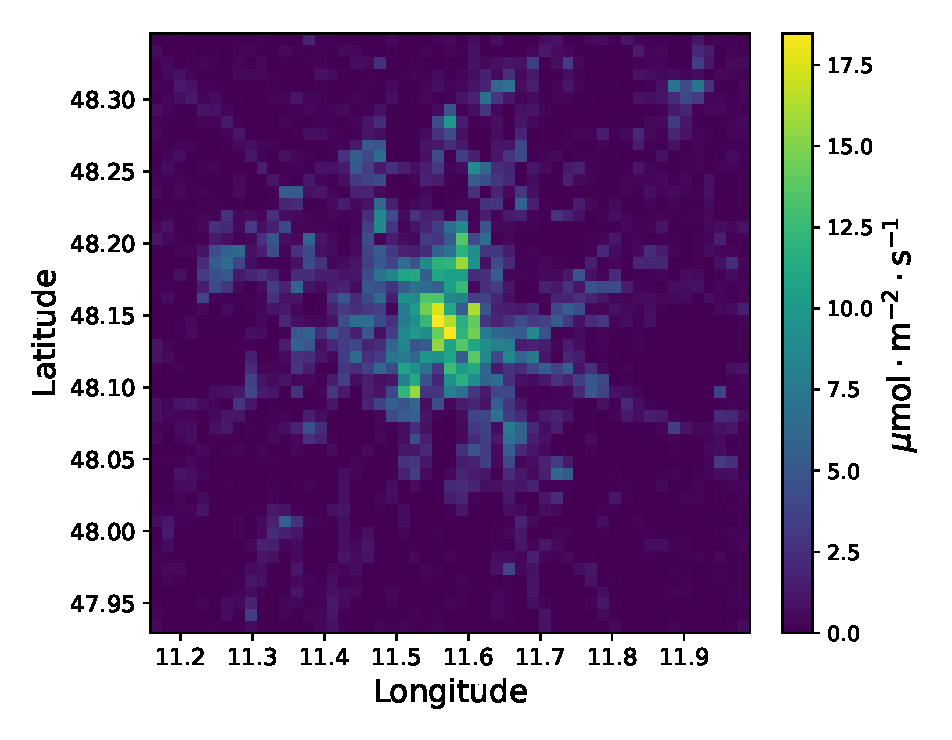
\includegraphics[width=\linewidth]{figures/03_dataset/munich/munich_2015_total_emissions.eps}
        \caption{Total Emission Fluxes}
    \end{subfigure}
    \begin{subfigure}{0.32\textwidth}
        \centering
        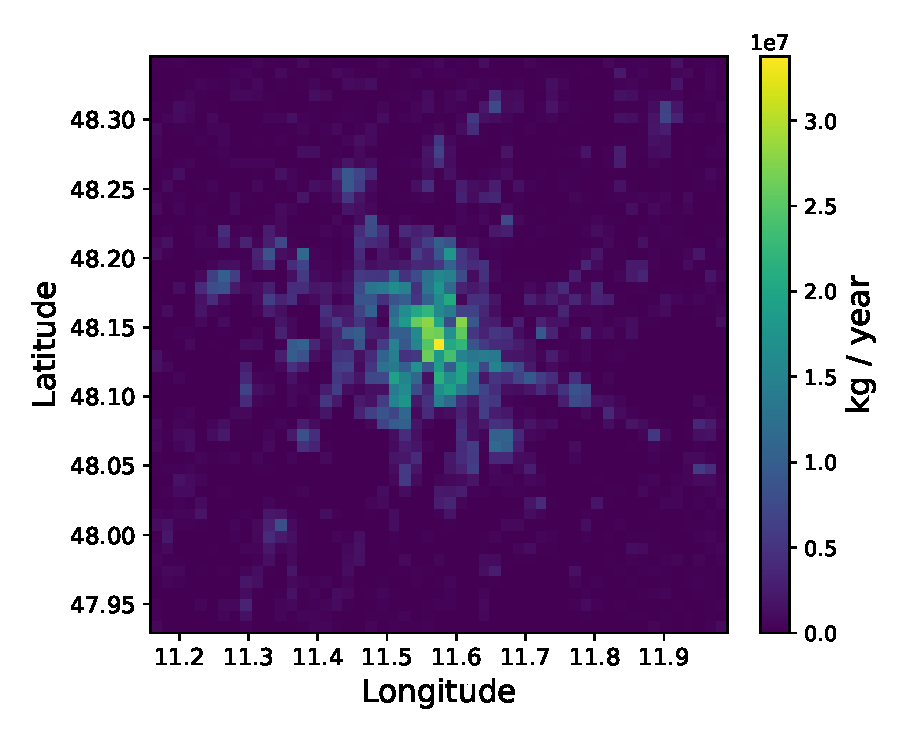
\includegraphics[width=\linewidth]{figures/03_dataset/munich/munich_2015_sector_c.eps}
        \caption{GNFR Sector C}
    \end{subfigure}
    \begin{subfigure}{0.32\textwidth}
        \centering
        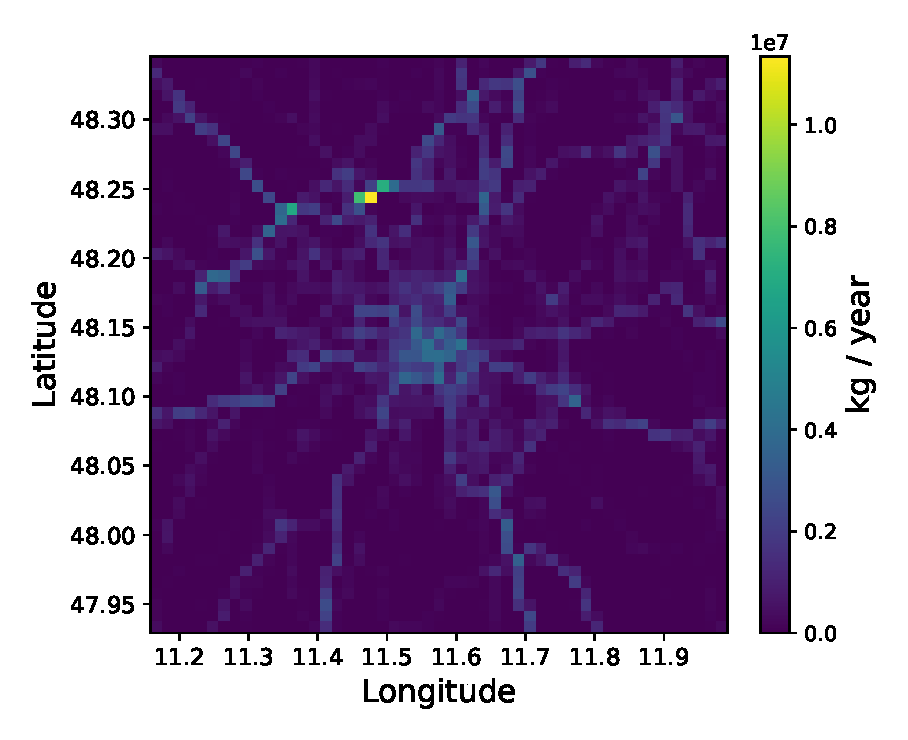
\includegraphics[width=\linewidth]{figures/03_dataset/munich/munich_2015_sector_f1.eps}
        \caption{GNFR Sector F1}
    \end{subfigure}
    \caption{$\text{CO}_2$ (ff) Emission Fluxes from Area Sources in Munich in 2015 \parencite{TNO_HighRes15}}
    \label{fig:munich_emissions}
\end{figure}
Therefore, as this thesis focuses on urban environments, they have to be filtered from the TNO-GHGco datasets.
For this, several cities are selected from a public database by OpenDatasoft \parencite{OpenDataSoft}.
Cities are filtered according to their population size.
For this thesis, we define a population threshold of $100,000$.
Any cities with a population greater than $100,000$ are selected for the dataset.

The coordinates of the filtered cities are then used to extract emission fields.
From the inventories, $51$ by $51$ grid cells around the city center are extracted.
This corresponds to a dimension of approximately $51 \unit{km}$ by $51 \unit{km}$. 
While most cities are not even close to this size, this allows for later cropping of the fields to a desired size.
For this thesis, emission fields have a final size of $32$ by $32$.

Some cities may be too close to each other, resulting in data leakage to test and validation sets.
Thus, cities are filtered if they are too close to other cities.
The following algorithm guarantees that no cities in the dataset overlap.

\begin{quotation}
First, an empty list of extracted lists is initialized.
Then, for each city, the latitude and longitude distances to all extracted cities are calculated.
In the next step, the algorithm determines which cities fall within a defined distance threshold from the current city.
If no cities are found within this threshold, the current city is added to the list, and the algorithm moves on to the next city.
However, if overlapping cities are identified within the threshold, the population size of the current city is compared to those of the overlapping cities.
If the current city has a larger population than all of the overlapping cities, these cities are removed, and the current city is added to the list.
If the current city does not have a larger population, it is ignored, and the algorithm continues with the next city.
\end{quotation}

This extraction results in $106$ city emission fields per year, $2015$, and $2018$.
However, we identified Bratislava as an outlier for this dataset due to its high \gls{SSIM} with a $0$ emission field.
Therefore, we exclude Bratislava from the dataset, thus reducing the number of cities to $105$.

This limited number of extracted emission fields is insufficient to train a generative model.
Thus, temporal scaling factors from \parencite{ScalingFactors} are useful for artificially generating more samples.
Scaling factors are applied to individual GNFR sectors.
This results in $24 \cdot 7 \cdot 12 = 2016$ samples per city per year.
The resulting combined dataset size is then $105 \cdot 2 \cdot 2016 = 423,360$ individual emission fields with size $51$ by $51$.
Scaling factors are applied at sampling time to reduce memory overhead, thus only keeping the original data in memory.

\section{Dataset Split}
The emission fields are divided into training, validation, and test sets.
The test set comprises $t$ percent of the data and is used exclusively for experiments and evaluations; the model does not encounter this data during training.
The validation set makes up $v$ percent of the data and is used during training to assess the model's generalization capabilities.
The remaining data, i.e., $1-v-t$ percent, is allocated to the training set for updating the model's weights.

A random split could result in unrepresentative subsets since emission fields of cities may vary significantly in their mean emissions.
For example, if the validation set contains cities with higher mean emissions, the \gls{MSE} during validation would be higher due to \gls{MSE}'s sensitivity to scale.
Therefore, it is essential to distribute cities equally across the training, validation, and test sets concerning their mean emissions to best assess generalization abilities.
Additionally, data from individual cities should not be split across different datasets to prevent data leakage.
For instance, Berlin's data from $2015$ should not be in the test set if its $2018$ data is in the training set.

The following algorithm fulfills both requirements from above while producing a reproducible split:

\begin{quotation}
First, the algorithm groups the emission fields according to their city name.
The emission fields are then sorted alphabetically according to the above names.
In the second step, the algorithm sorts the emission fields by their mean emissions in descending order.
Finally, it splits the dataset using equidistant indices to produce two datasets.
\end{quotation}

This algorithm is then used to assign $t$ percent of the data to the test set.
Then, from the remaining $1 - t$ percent, $\frac{v}{1 - t}$ percent is assigned to the validation set.
The rest is allocated to the training set.

\section{Data Augmentation}
To enhance the generalization capabilities of the model, we apply common image augmentation \parencite{ImageAugmentation} to the emission fields in the training dataset.
The augmentation methods applied include random cropping, flipping, and rotation.
To introduce variability in spatial positioning, emission fields are randomly cropped to a spatial dimension of $32$ by $32$.
Additionally, with a probability of $0.5$, the emission fields undergo horizontal or vertical flipping.
Similarly, with a probability of $0.5$, they are rotated by $90$ degrees.
These techniques result in eight possible transformations for each emission field, including the original unaltered version.

An example of this augmentation process is illustrated in Figure \ref{fig:nuernberg_emissions}.
The figure shows the original and transformed emission fields for the Nuremberg area sources, highlighting how the summed emissions are altered through the applied transformations.

\begin{figure}[h!]
    \centering
    \begin{subfigure}{0.4\textwidth}
        \centering
        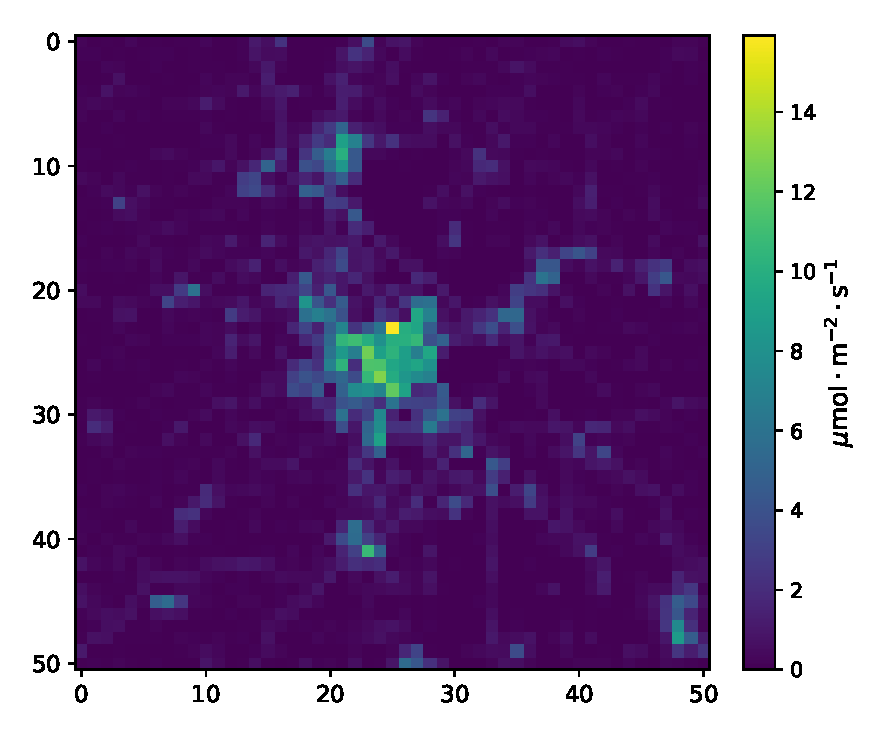
\includegraphics[width=\linewidth]{figures/03_dataset/nuernberg/nuernberg.eps}
        \caption{Original}
    \end{subfigure}
    \begin{subfigure}{0.4\textwidth}
        \centering
        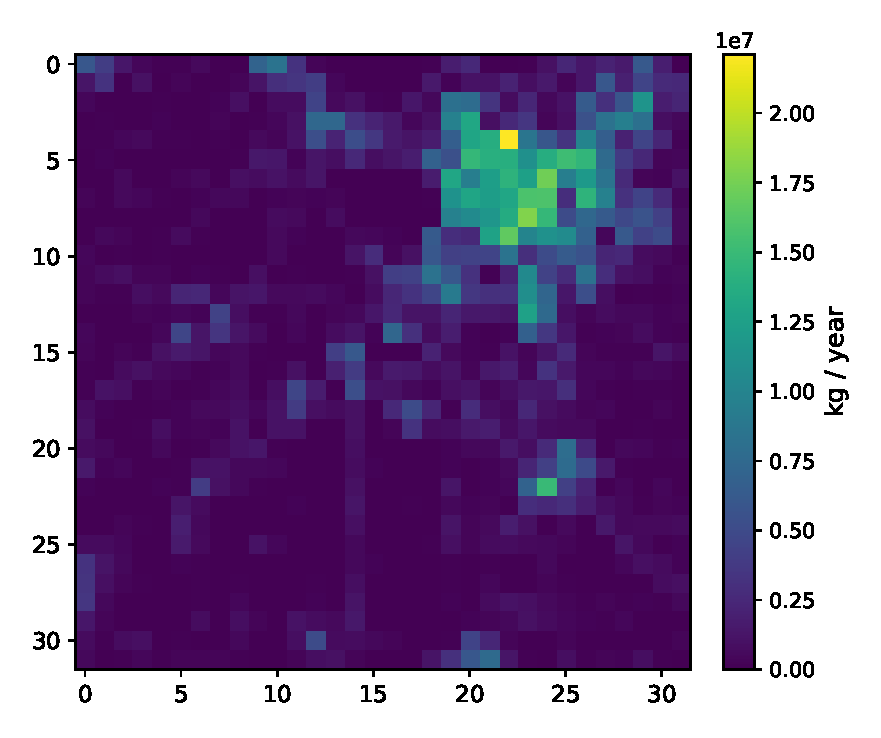
\includegraphics[width=\linewidth]{figures/03_dataset/nuernberg/nuernberg_transformed.eps}
        \caption{Transformed}
    \end{subfigure}
    \caption{Total $\text{CO}_2$ (ff) Emission Fluxes from Area Sources in Nuremberg in 2015 \parencite{TNO_HighRes15}}
    \label{fig:nuernberg_emissions}
\end{figure}

It is important to note that these transformations are not applied to the validation and test emission fields, except for a center crop to match the expected input dimensions.

\section{Scaling}
Scaling plays an important role in machine learning.
Large-scale data can make training converge slowly and become unstable \parencite{DataScaling}.
A common technique for scaling values is min-max scaling \parencite{MinMaxScaling}.
However, min-max scaling is sensitive to outliers and thus not ideal for emission inventories where the range of emissions within a city can vary greatly.
Instead, robust scaling can be applied.
To determine a good scaling factor, the $95$th percentile of values is determined for each city in the training set.
The inverse of the average is then used as the scaling factor.
The resulting scaling factor is thus $\frac{1}{2.5 * 10^6}$ after rounding.
All experiments are, without loss of generality, performed on the scaled data.

\section{Case Studies}
In addition to the test data used for model performance evaluation, three cities are selected for detailed case studies.
The cities are Munich, Zurich, and Paris.
These cities are chosen based on the ICOS Cities PAUL project \parencite{Icos} and represent a range of city sizes, from small to medium and large.
In order to ensure unbiased results, these cities are excluded from the dataset prior to splitting, reducing the total number of cities available for training from $105$ to $102$.
These cities allow closer inspection of the outputs of different algorithms.
